% Appendix: remaining routing analysis (not in the main heatmap / Sec.~5.6).
% Copy the PNGs into your paper figures/ folder and % Appendix: remaining routing analysis (not in the main heatmap / Sec.~5.6).
% Copy the PNGs into your paper figures/ folder and % Appendix: remaining routing analysis (not in the main heatmap / Sec.~5.6).
% Copy the PNGs into your paper figures/ folder and % Appendix: remaining routing analysis (not in the main heatmap / Sec.~5.6).
% Copy the PNGs into your paper figures/ folder and \input{appendix_routing}.

\section{Additional routing analysis}
\label{app:routing}

The main paper reports only the \emph{final} color-leaf mass heatmap.
This appendix records how that assignment is reached: gate entropy over
training, a single-scene growth trace, and final entropy / utilization
statistics. All plots use the color head.
Logs are written every 1k iterations to \texttt{routing\_analysis.json}.
Sample entropy \(H\) is in nats (uniform over 8 experts is \(\ln 8 \approx 2.08\)).

\subsection{Entropy over training}
\label{app:routing-entropy}

Figure~\ref{fig:app-entropy} shows color-head sample entropy versus
iteration on Mip-NeRF~360. Flat MoE uses a dense softmax for the first
\(T_{\mathrm{w}}{=}3000\) iterations, so \(H\) sits near \(2.08\), then
collapses after Top-2 turns on. Tree MoE is warm-started from the Stage~A
checkpoint, so it never revisits that dense plateau: \(H\) stays near zero,
with a small bump at the start of Stage~B and faint rises after grow
checks (dashed, \(t\in\{6\mathrm{k},10\mathrm{k},14\mathrm{k},18\mathrm{k}\}\)).
The same curves on Tanks~\&~Temples, Deep Blending, and NeRF-Synthetic
are Figs.~\ref{fig:entropy-tandt}--\ref{fig:entropy-nerf}.
\texttt{train} keeps the highest residual flat-MoE entropy (\(H{=}0.100\));
the tree still halves it.

\begin{figure}[t]
  \centering
  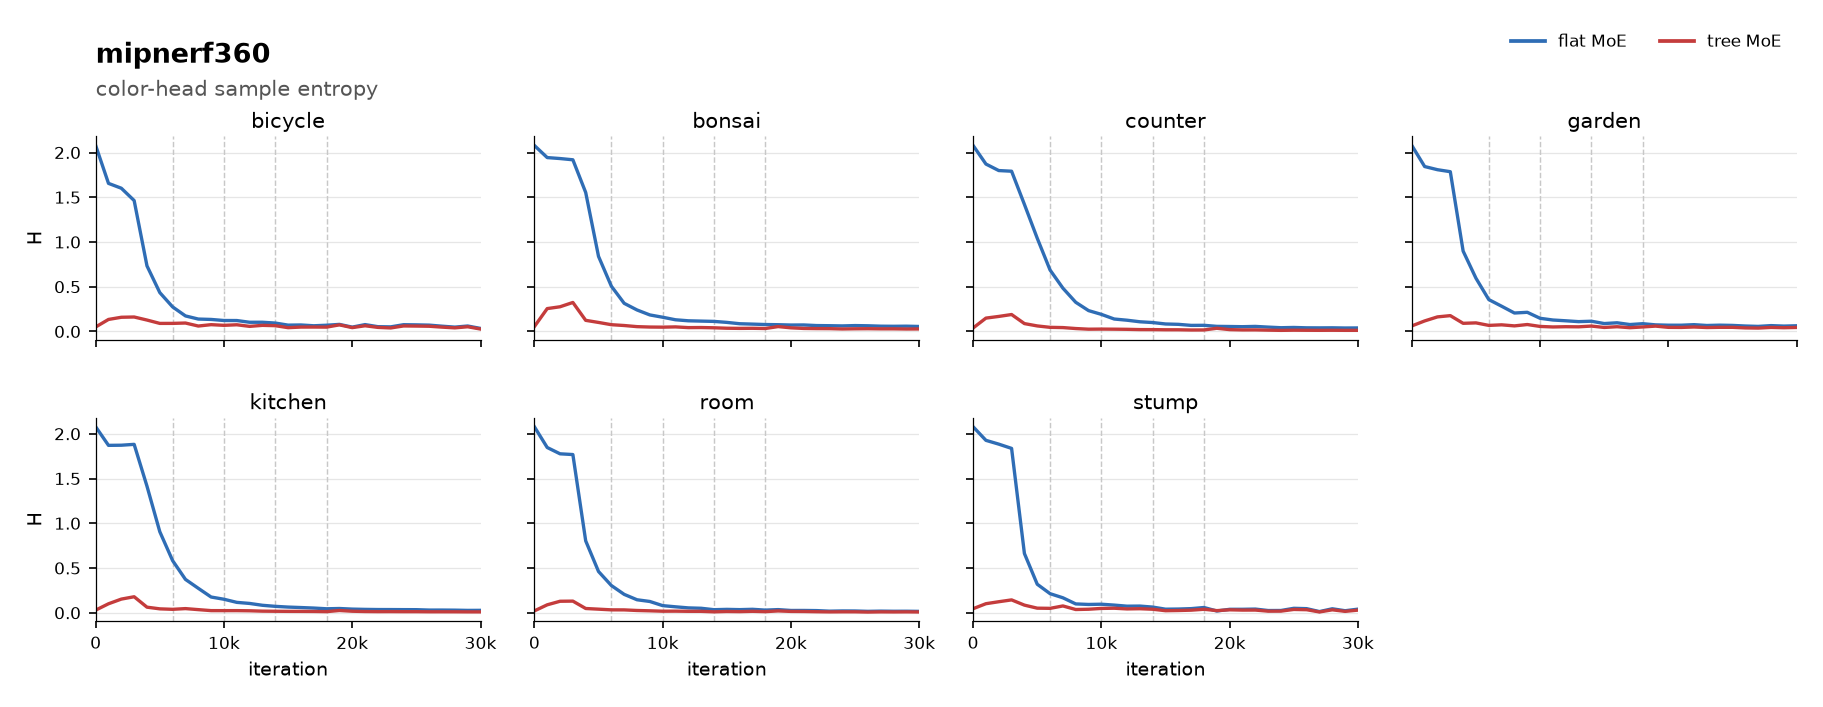
\includegraphics[width=\linewidth]{figures/mipnerf360__entropy_grid.png}
  \caption{\textbf{Color-head sample entropy over training} (Mip-NeRF~360).
  Blue: flat MoE. Red: tree MoE. Shared \(y\)-axis.
  Flat MoE shows the dense-warmup plateau then a Top-2 collapse;
  tree MoE remains specialized throughout Stage~B.}
  \label{fig:app-entropy}
\end{figure}

\begin{figure}[t]
  \centering
  \includegraphics[width=\linewidth]{tandt__entropy_grid.png}
  \caption{Color-head sample entropy \(H\) versus iteration on Tanks~\&~Temples
  (\texttt{train}, \texttt{truck}).
  Blue: flat MoE (dense softmax for \(3\mathrm{k}\) iterations, then Top-2).
  Red: tree MoE warm-started from Stage~A; dashed lines are growth checks.
  Flat MoE collapses after warm-up; tree MoE stays near \(H{\approx}0\).
  \texttt{train} is the slowest collapse and the highest residual entropy.}
  \label{fig:entropy-tandt}
\end{figure}

\begin{figure}[t]
  \centering
  \includegraphics[width=\linewidth]{db__entropy_grid.png}
  \caption{Color-head sample entropy \(H\) versus iteration on Deep Blending
  (\texttt{drjohnson}, \texttt{playroom}).
  Blue: flat MoE. Red: tree MoE. Shared \(y\)-axis in nats
  (uniform over 8 experts is \(\ln 8\approx 2.08\)).
  Both indoor scenes follow the same curriculum: a dense-warmup plateau,
  then a Top-2 collapse.
  Tree MoE never revisits that plateau; \texttt{playroom} keeps a slightly
  higher residual \(H\) than \texttt{drjohnson}.}
  \label{fig:entropy-db}
\end{figure}

\begin{figure}[t]
  \centering
  \includegraphics[width=\linewidth]{nerfsynthetic__entropy_grid.png}
  \caption{Color-head sample entropy \(H\) versus iteration on all eight
  NeRF-Synthetic scenes.
  Blue: flat MoE. Red: tree MoE.
  Every object shows the same pattern as the real scenes: flat MoE sits near
  \(H{\approx}2\) during warm-up and then specializes, while tree MoE remains
  specialized for the whole \(30\mathrm{k}\) Stage~B run.}
  \label{fig:entropy-nerf}
\end{figure}

\subsection{Growth trace on \texttt{kitchen}}
\label{app:routing-kitchen}

Figure~\ref{fig:app-kitchen} is the per-scene dump for \texttt{kitchen}
(\(+1.00\)\,dB vs.\ Scaffold-GS, \(+0.53\)\,dB vs.\ flat MoE).
The middle row is routing mass versus iteration.
Gray cells are leaves that do not exist yet; new columns appear at grow
events. After a split the parent goes dark and the two children inherit
its mass. On \texttt{kitchen} the color head splits \(L_{6,7}\) at 6k and
\(L_{0,1}\) at 10k, ending at 11 leaves, one of which is unused.
The top row is entropy (baseline is the shared MLP, \(H{=}0\));
the bottom row is the 30k mass histogram (same information as one row of
the main heatmap). Bonsai is the other high-gain scene and shows a
stronger flat-MoE collapse (CV \(0.87\), two experts hold most of the mass).

\begin{figure}[t]
  \centering
  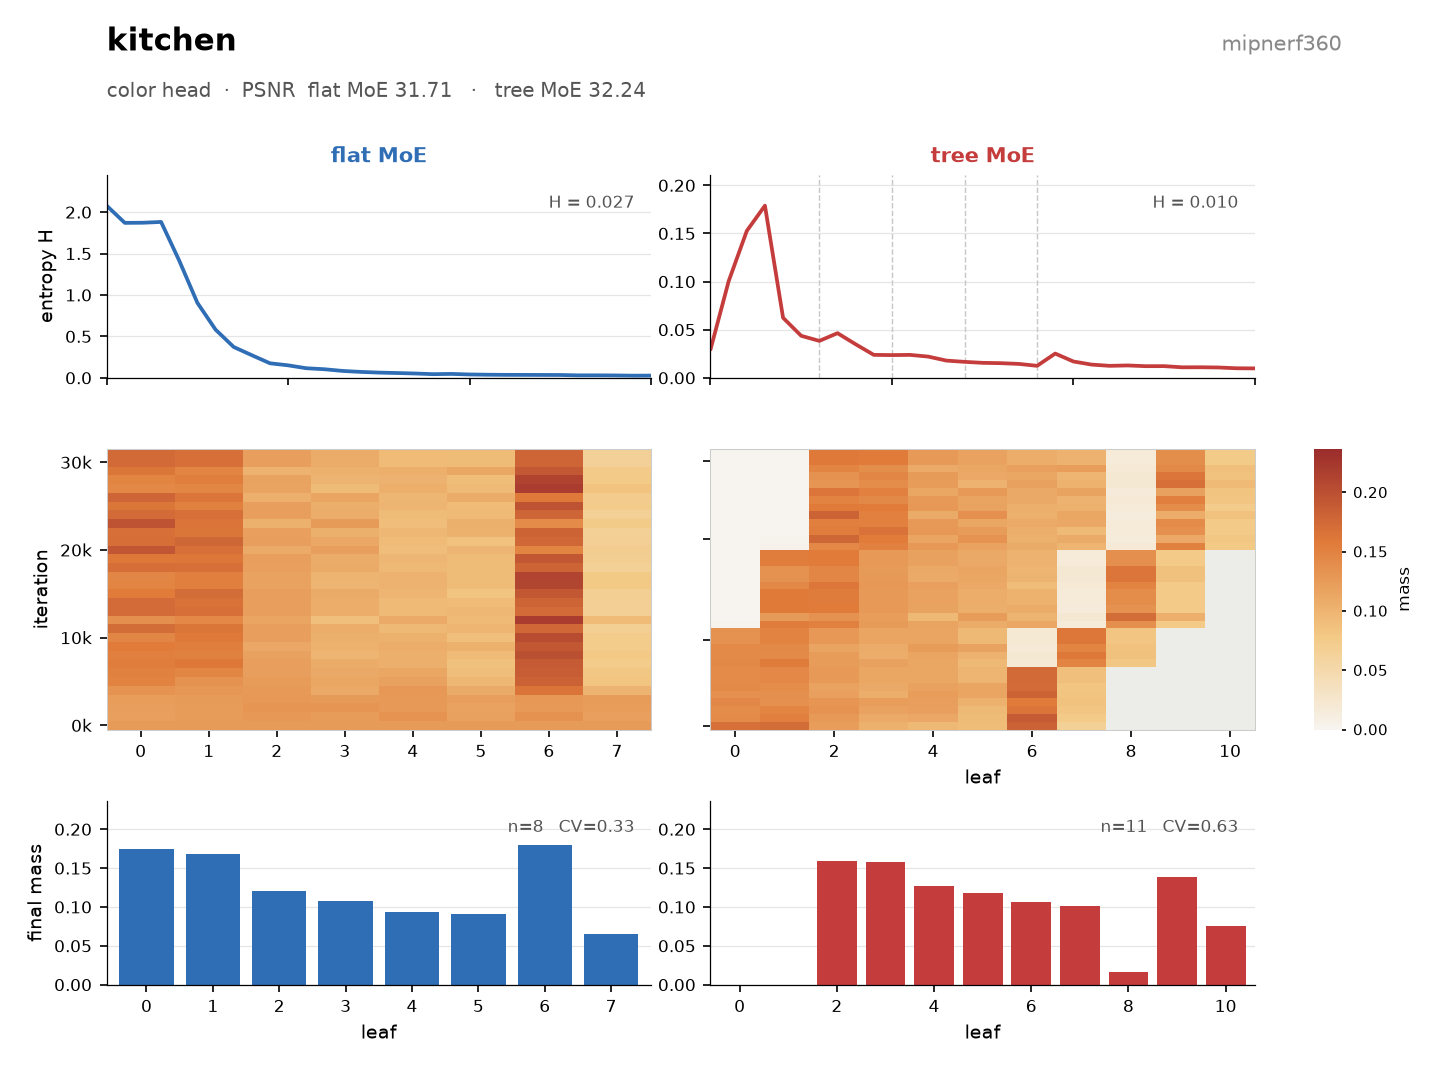
\includegraphics[width=\linewidth]{figures/kitchen.png}
  \caption{\textbf{Per-scene routing dump on \texttt{kitchen}.}
  Columns: flat MoE, tree MoE (color head).
  Top: sample entropy. Middle: leaf mass over training
  (gray \(=\) not yet grown). Bottom: final mass, leaf count \(n\), and
  utilization CV.}
  \label{fig:app-kitchen}
\end{figure}

\subsection{Final entropy and utilization}
\label{app:routing-final}

Figure~\ref{fig:app-hcv} summarizes the 30k color-head statistics on all
19 scenes. Tree MoE has \emph{lower} sample entropy than flat MoE on every
scene, even though it has more leaves (11 vs.\ 8): the extra capacity is
used as specialists, not as a more uniform mixture.
Utilization CV is mixed and should not be read as ``tree is more balanced.''
Flat MoE is sometimes peaked (\texttt{room}, \texttt{bonsai}, CV \(\ge 0.85\))
and sometimes flatter (\texttt{kitchen}, \texttt{garden}).
Tree CV lies in a narrower band, roughly \(0.5\)--\(0.7\), because splits
move mass onto children and leave some parents empty.

Opacity routers stay slightly higher-entropy than color; covariance
collapses first. We therefore report color in the main paper as the head
that actually paints the image.

\begin{figure}[t]
  \centering
  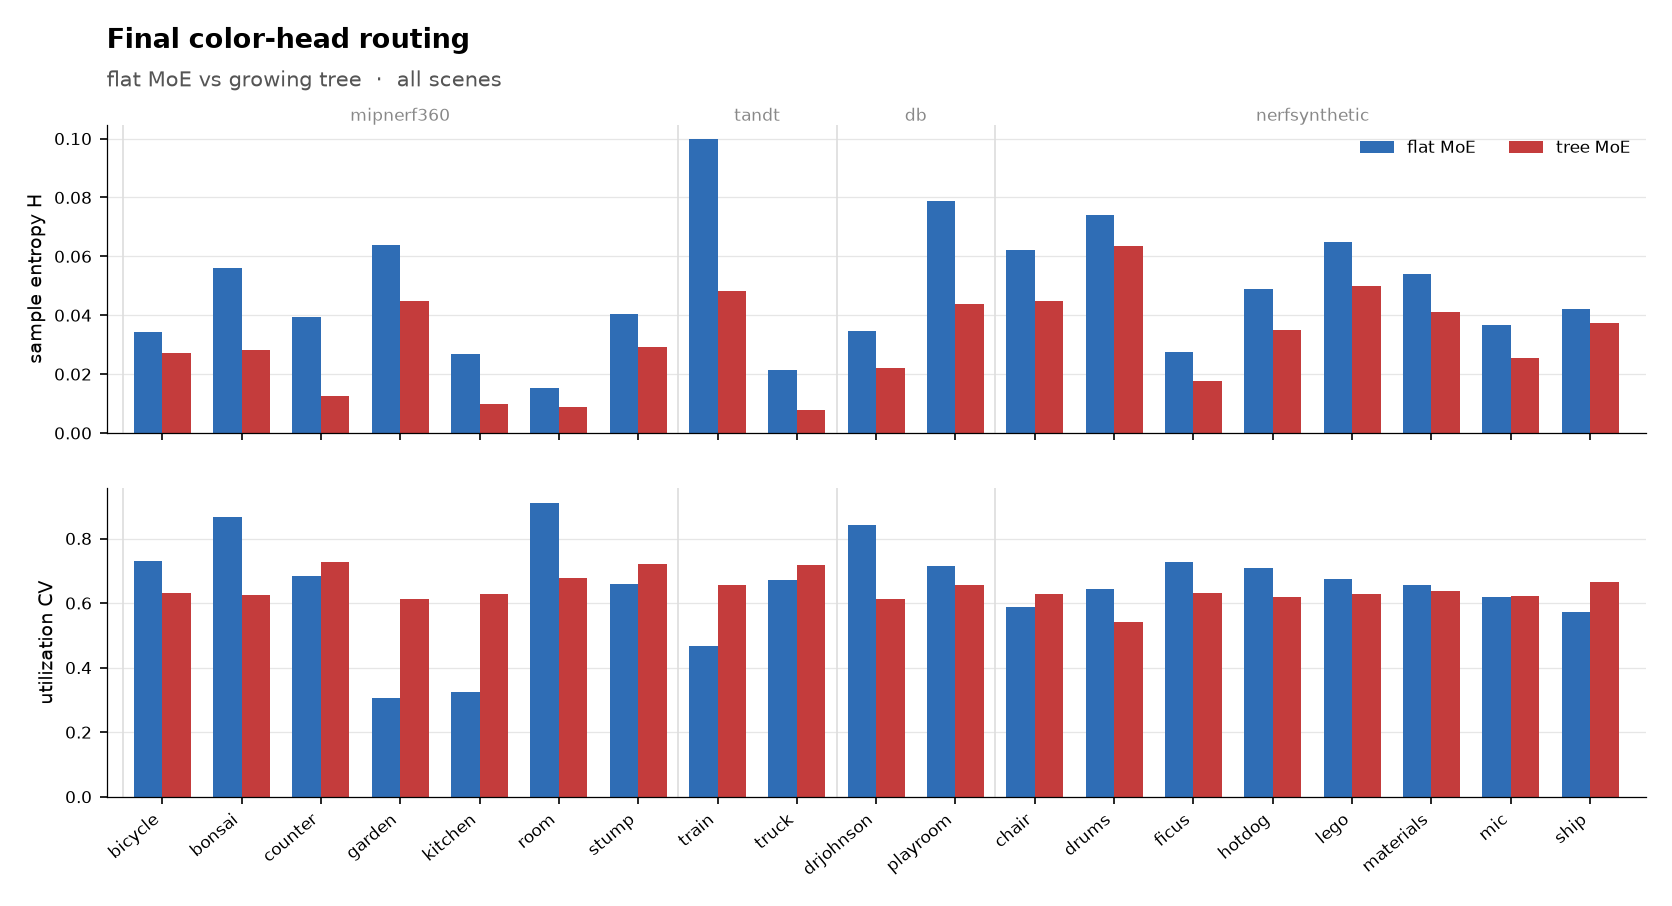
\includegraphics[width=\linewidth]{figures/all_scenes__final_metrics.png}
  \caption{\textbf{Final color-head entropy and utilization CV} (19 scenes).
  Top: sample entropy \(H\); tree \(<\) flat on every scene.
  Bottom: utilization CV (0 \(=\) equal mass). Tree CV is steadier;
  flat MoE oscillates between collapse and near-uniform use of the 8 experts.}
  \label{fig:app-hcv}
\end{figure}

These traces are consistent with Sec.~\ref{sec:grow-ablate}:
\(G_{\max}{=}0\) already captures most of the PSNR gain.
Growth reallocates capacity and makes that specialization readable;
it is not required for the mean \(+0.30\)\,dB over flat MoE.
.

\section{Additional routing analysis}
\label{app:routing}

The main paper reports only the \emph{final} color-leaf mass heatmap.
This appendix records how that assignment is reached: gate entropy over
training, a single-scene growth trace, and final entropy / utilization
statistics. All plots use the color head.
Logs are written every 1k iterations to \texttt{routing\_analysis.json}.
Sample entropy \(H\) is in nats (uniform over 8 experts is \(\ln 8 \approx 2.08\)).

\subsection{Entropy over training}
\label{app:routing-entropy}

Figure~\ref{fig:app-entropy} shows color-head sample entropy versus
iteration on Mip-NeRF~360. Flat MoE uses a dense softmax for the first
\(T_{\mathrm{w}}{=}3000\) iterations, so \(H\) sits near \(2.08\), then
collapses after Top-2 turns on. Tree MoE is warm-started from the Stage~A
checkpoint, so it never revisits that dense plateau: \(H\) stays near zero,
with a small bump at the start of Stage~B and faint rises after grow
checks (dashed, \(t\in\{6\mathrm{k},10\mathrm{k},14\mathrm{k},18\mathrm{k}\}\)).
The same curves on Tanks~\&~Temples, Deep Blending, and NeRF-Synthetic
are Figs.~\ref{fig:entropy-tandt}--\ref{fig:entropy-nerf}.
\texttt{train} keeps the highest residual flat-MoE entropy (\(H{=}0.100\));
the tree still halves it.

\begin{figure}[t]
  \centering
  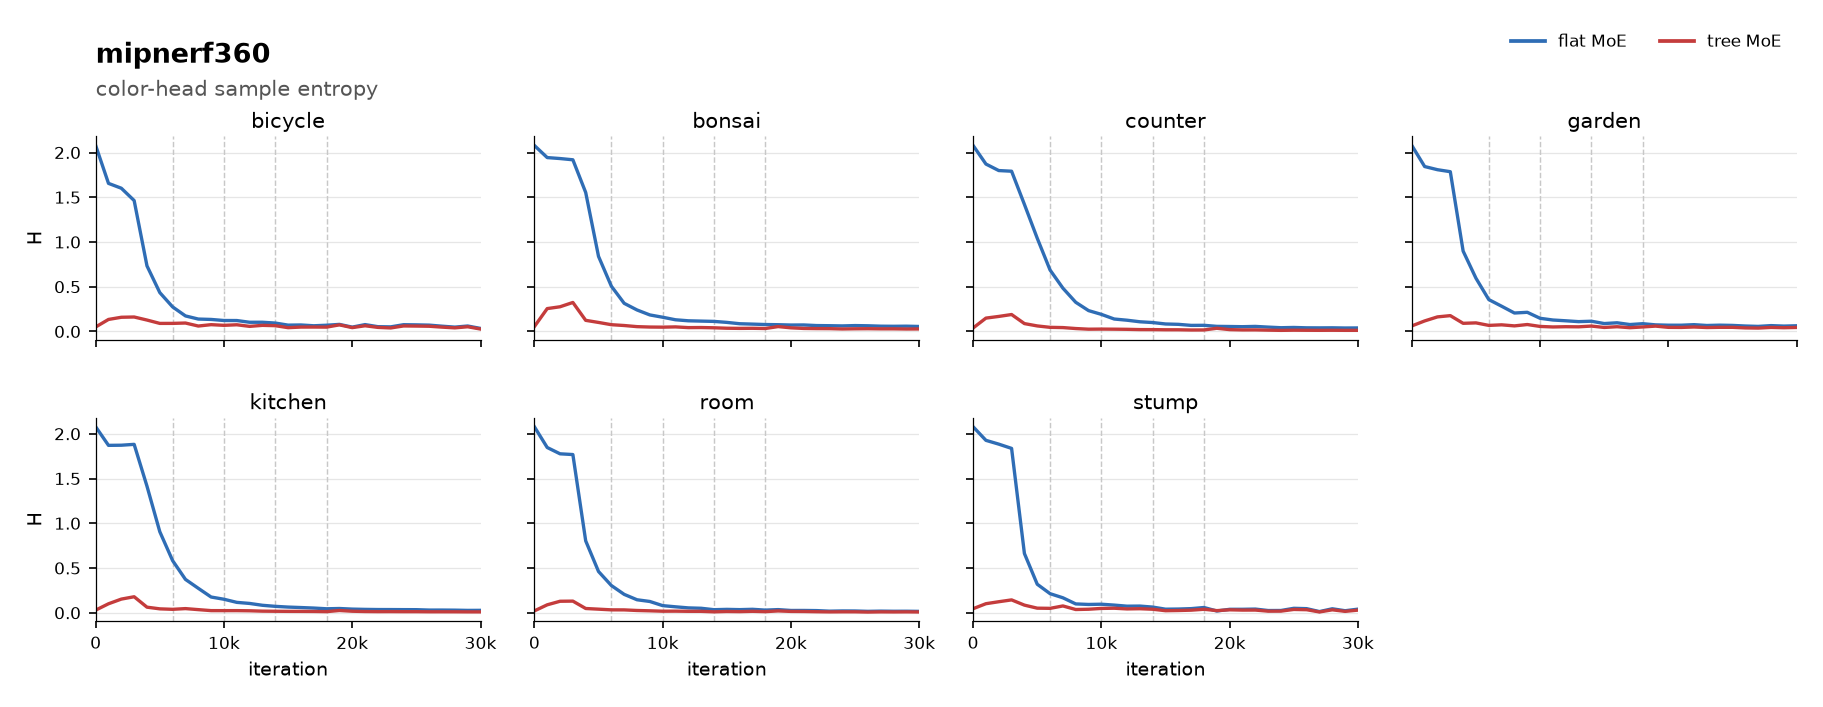
\includegraphics[width=\linewidth]{figures/mipnerf360__entropy_grid.png}
  \caption{\textbf{Color-head sample entropy over training} (Mip-NeRF~360).
  Blue: flat MoE. Red: tree MoE. Shared \(y\)-axis.
  Flat MoE shows the dense-warmup plateau then a Top-2 collapse;
  tree MoE remains specialized throughout Stage~B.}
  \label{fig:app-entropy}
\end{figure}

\begin{figure}[t]
  \centering
  \includegraphics[width=\linewidth]{tandt__entropy_grid.png}
  \caption{Color-head sample entropy \(H\) versus iteration on Tanks~\&~Temples
  (\texttt{train}, \texttt{truck}).
  Blue: flat MoE (dense softmax for \(3\mathrm{k}\) iterations, then Top-2).
  Red: tree MoE warm-started from Stage~A; dashed lines are growth checks.
  Flat MoE collapses after warm-up; tree MoE stays near \(H{\approx}0\).
  \texttt{train} is the slowest collapse and the highest residual entropy.}
  \label{fig:entropy-tandt}
\end{figure}

\begin{figure}[t]
  \centering
  \includegraphics[width=\linewidth]{db__entropy_grid.png}
  \caption{Color-head sample entropy \(H\) versus iteration on Deep Blending
  (\texttt{drjohnson}, \texttt{playroom}).
  Blue: flat MoE. Red: tree MoE. Shared \(y\)-axis in nats
  (uniform over 8 experts is \(\ln 8\approx 2.08\)).
  Both indoor scenes follow the same curriculum: a dense-warmup plateau,
  then a Top-2 collapse.
  Tree MoE never revisits that plateau; \texttt{playroom} keeps a slightly
  higher residual \(H\) than \texttt{drjohnson}.}
  \label{fig:entropy-db}
\end{figure}

\begin{figure}[t]
  \centering
  \includegraphics[width=\linewidth]{nerfsynthetic__entropy_grid.png}
  \caption{Color-head sample entropy \(H\) versus iteration on all eight
  NeRF-Synthetic scenes.
  Blue: flat MoE. Red: tree MoE.
  Every object shows the same pattern as the real scenes: flat MoE sits near
  \(H{\approx}2\) during warm-up and then specializes, while tree MoE remains
  specialized for the whole \(30\mathrm{k}\) Stage~B run.}
  \label{fig:entropy-nerf}
\end{figure}

\subsection{Growth trace on \texttt{kitchen}}
\label{app:routing-kitchen}

Figure~\ref{fig:app-kitchen} is the per-scene dump for \texttt{kitchen}
(\(+1.00\)\,dB vs.\ Scaffold-GS, \(+0.53\)\,dB vs.\ flat MoE).
The middle row is routing mass versus iteration.
Gray cells are leaves that do not exist yet; new columns appear at grow
events. After a split the parent goes dark and the two children inherit
its mass. On \texttt{kitchen} the color head splits \(L_{6,7}\) at 6k and
\(L_{0,1}\) at 10k, ending at 11 leaves, one of which is unused.
The top row is entropy (baseline is the shared MLP, \(H{=}0\));
the bottom row is the 30k mass histogram (same information as one row of
the main heatmap). Bonsai is the other high-gain scene and shows a
stronger flat-MoE collapse (CV \(0.87\), two experts hold most of the mass).

\begin{figure}[t]
  \centering
  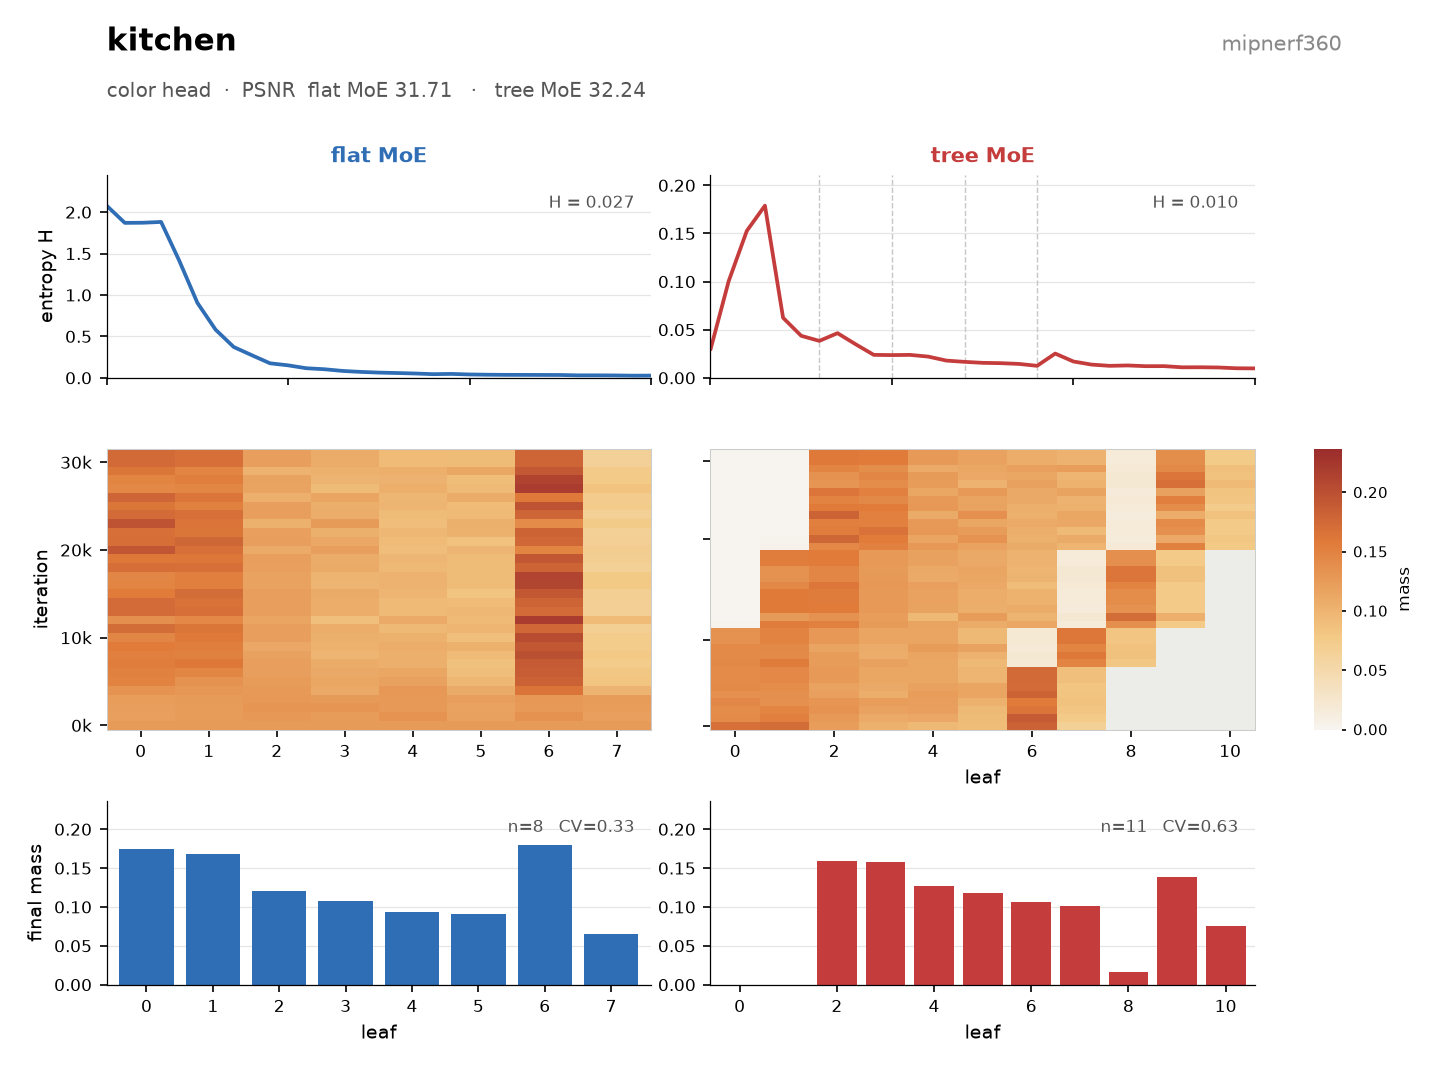
\includegraphics[width=\linewidth]{figures/kitchen.png}
  \caption{\textbf{Per-scene routing dump on \texttt{kitchen}.}
  Columns: flat MoE, tree MoE (color head).
  Top: sample entropy. Middle: leaf mass over training
  (gray \(=\) not yet grown). Bottom: final mass, leaf count \(n\), and
  utilization CV.}
  \label{fig:app-kitchen}
\end{figure}

\subsection{Final entropy and utilization}
\label{app:routing-final}

Figure~\ref{fig:app-hcv} summarizes the 30k color-head statistics on all
19 scenes. Tree MoE has \emph{lower} sample entropy than flat MoE on every
scene, even though it has more leaves (11 vs.\ 8): the extra capacity is
used as specialists, not as a more uniform mixture.
Utilization CV is mixed and should not be read as ``tree is more balanced.''
Flat MoE is sometimes peaked (\texttt{room}, \texttt{bonsai}, CV \(\ge 0.85\))
and sometimes flatter (\texttt{kitchen}, \texttt{garden}).
Tree CV lies in a narrower band, roughly \(0.5\)--\(0.7\), because splits
move mass onto children and leave some parents empty.

Opacity routers stay slightly higher-entropy than color; covariance
collapses first. We therefore report color in the main paper as the head
that actually paints the image.

\begin{figure}[t]
  \centering
  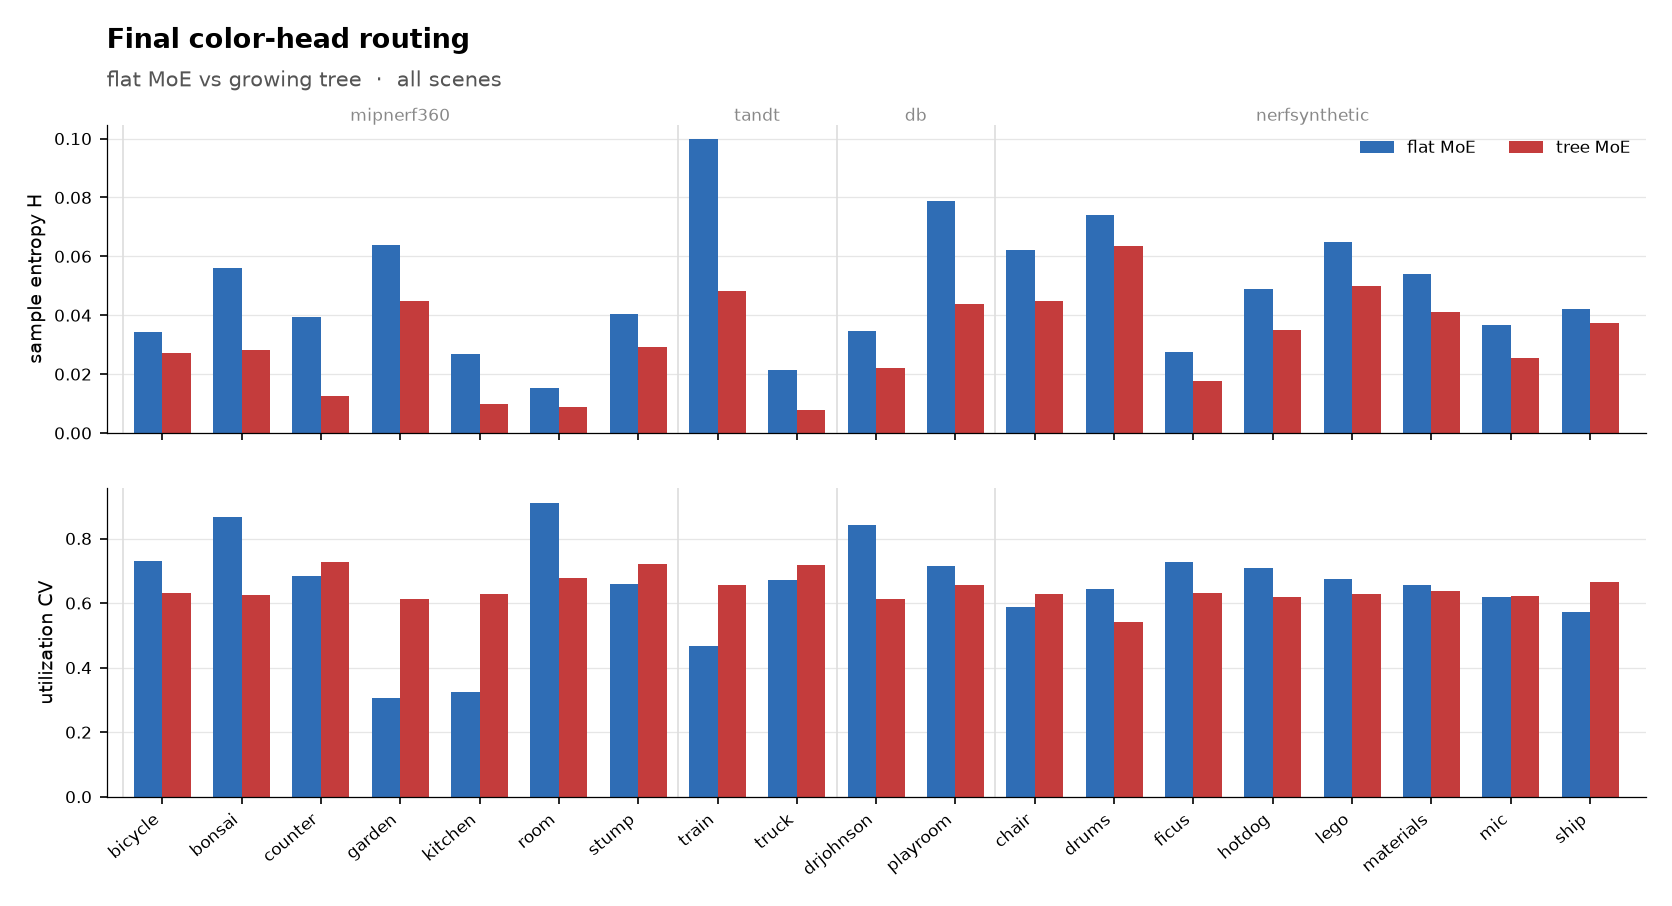
\includegraphics[width=\linewidth]{figures/all_scenes__final_metrics.png}
  \caption{\textbf{Final color-head entropy and utilization CV} (19 scenes).
  Top: sample entropy \(H\); tree \(<\) flat on every scene.
  Bottom: utilization CV (0 \(=\) equal mass). Tree CV is steadier;
  flat MoE oscillates between collapse and near-uniform use of the 8 experts.}
  \label{fig:app-hcv}
\end{figure}

These traces are consistent with Sec.~\ref{sec:grow-ablate}:
\(G_{\max}{=}0\) already captures most of the PSNR gain.
Growth reallocates capacity and makes that specialization readable;
it is not required for the mean \(+0.30\)\,dB over flat MoE.
.

\section{Additional routing analysis}
\label{app:routing}

The main paper reports only the \emph{final} color-leaf mass heatmap.
This appendix records how that assignment is reached: gate entropy over
training, a single-scene growth trace, and final entropy / utilization
statistics. All plots use the color head.
Logs are written every 1k iterations to \texttt{routing\_analysis.json}.
Sample entropy \(H\) is in nats (uniform over 8 experts is \(\ln 8 \approx 2.08\)).

\subsection{Entropy over training}
\label{app:routing-entropy}

Figure~\ref{fig:app-entropy} shows color-head sample entropy versus
iteration on Mip-NeRF~360. Flat MoE uses a dense softmax for the first
\(T_{\mathrm{w}}{=}3000\) iterations, so \(H\) sits near \(2.08\), then
collapses after Top-2 turns on. Tree MoE is warm-started from the Stage~A
checkpoint, so it never revisits that dense plateau: \(H\) stays near zero,
with a small bump at the start of Stage~B and faint rises after grow
checks (dashed, \(t\in\{6\mathrm{k},10\mathrm{k},14\mathrm{k},18\mathrm{k}\}\)).
The same curves on Tanks~\&~Temples, Deep Blending, and NeRF-Synthetic
are Figs.~\ref{fig:entropy-tandt}--\ref{fig:entropy-nerf}.
\texttt{train} keeps the highest residual flat-MoE entropy (\(H{=}0.100\));
the tree still halves it.

\begin{figure}[t]
  \centering
  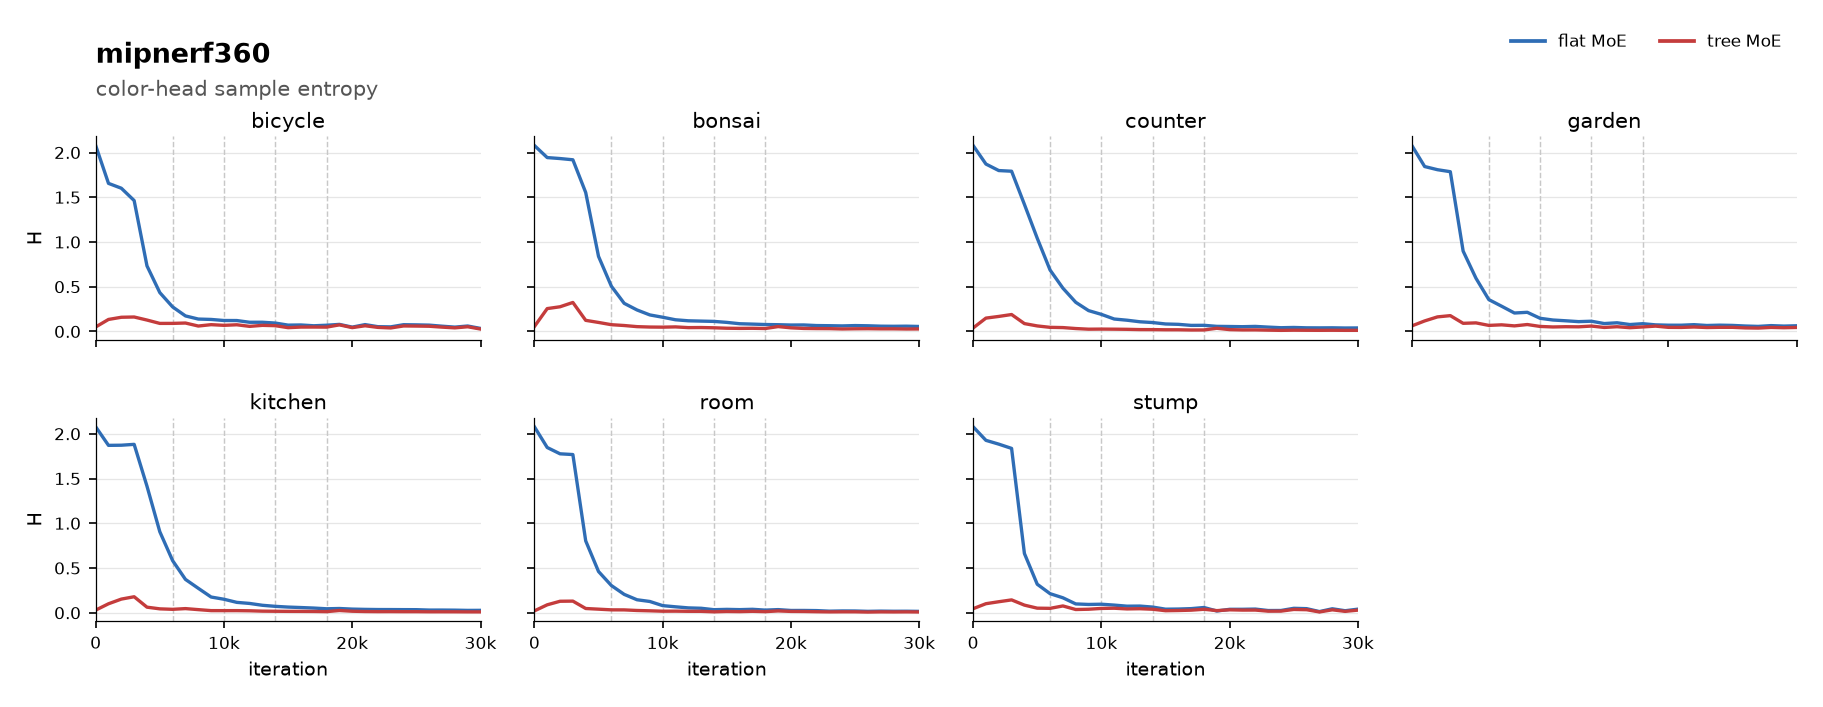
\includegraphics[width=\linewidth]{figures/mipnerf360__entropy_grid.png}
  \caption{\textbf{Color-head sample entropy over training} (Mip-NeRF~360).
  Blue: flat MoE. Red: tree MoE. Shared \(y\)-axis.
  Flat MoE shows the dense-warmup plateau then a Top-2 collapse;
  tree MoE remains specialized throughout Stage~B.}
  \label{fig:app-entropy}
\end{figure}

\begin{figure}[t]
  \centering
  \includegraphics[width=\linewidth]{tandt__entropy_grid.png}
  \caption{Color-head sample entropy \(H\) versus iteration on Tanks~\&~Temples
  (\texttt{train}, \texttt{truck}).
  Blue: flat MoE (dense softmax for \(3\mathrm{k}\) iterations, then Top-2).
  Red: tree MoE warm-started from Stage~A; dashed lines are growth checks.
  Flat MoE collapses after warm-up; tree MoE stays near \(H{\approx}0\).
  \texttt{train} is the slowest collapse and the highest residual entropy.}
  \label{fig:entropy-tandt}
\end{figure}

\begin{figure}[t]
  \centering
  \includegraphics[width=\linewidth]{db__entropy_grid.png}
  \caption{Color-head sample entropy \(H\) versus iteration on Deep Blending
  (\texttt{drjohnson}, \texttt{playroom}).
  Blue: flat MoE. Red: tree MoE. Shared \(y\)-axis in nats
  (uniform over 8 experts is \(\ln 8\approx 2.08\)).
  Both indoor scenes follow the same curriculum: a dense-warmup plateau,
  then a Top-2 collapse.
  Tree MoE never revisits that plateau; \texttt{playroom} keeps a slightly
  higher residual \(H\) than \texttt{drjohnson}.}
  \label{fig:entropy-db}
\end{figure}

\begin{figure}[t]
  \centering
  \includegraphics[width=\linewidth]{nerfsynthetic__entropy_grid.png}
  \caption{Color-head sample entropy \(H\) versus iteration on all eight
  NeRF-Synthetic scenes.
  Blue: flat MoE. Red: tree MoE.
  Every object shows the same pattern as the real scenes: flat MoE sits near
  \(H{\approx}2\) during warm-up and then specializes, while tree MoE remains
  specialized for the whole \(30\mathrm{k}\) Stage~B run.}
  \label{fig:entropy-nerf}
\end{figure}

\subsection{Growth trace on \texttt{kitchen}}
\label{app:routing-kitchen}

Figure~\ref{fig:app-kitchen} is the per-scene dump for \texttt{kitchen}
(\(+1.00\)\,dB vs.\ Scaffold-GS, \(+0.53\)\,dB vs.\ flat MoE).
The middle row is routing mass versus iteration.
Gray cells are leaves that do not exist yet; new columns appear at grow
events. After a split the parent goes dark and the two children inherit
its mass. On \texttt{kitchen} the color head splits \(L_{6,7}\) at 6k and
\(L_{0,1}\) at 10k, ending at 11 leaves, one of which is unused.
The top row is entropy (baseline is the shared MLP, \(H{=}0\));
the bottom row is the 30k mass histogram (same information as one row of
the main heatmap). Bonsai is the other high-gain scene and shows a
stronger flat-MoE collapse (CV \(0.87\), two experts hold most of the mass).

\begin{figure}[t]
  \centering
  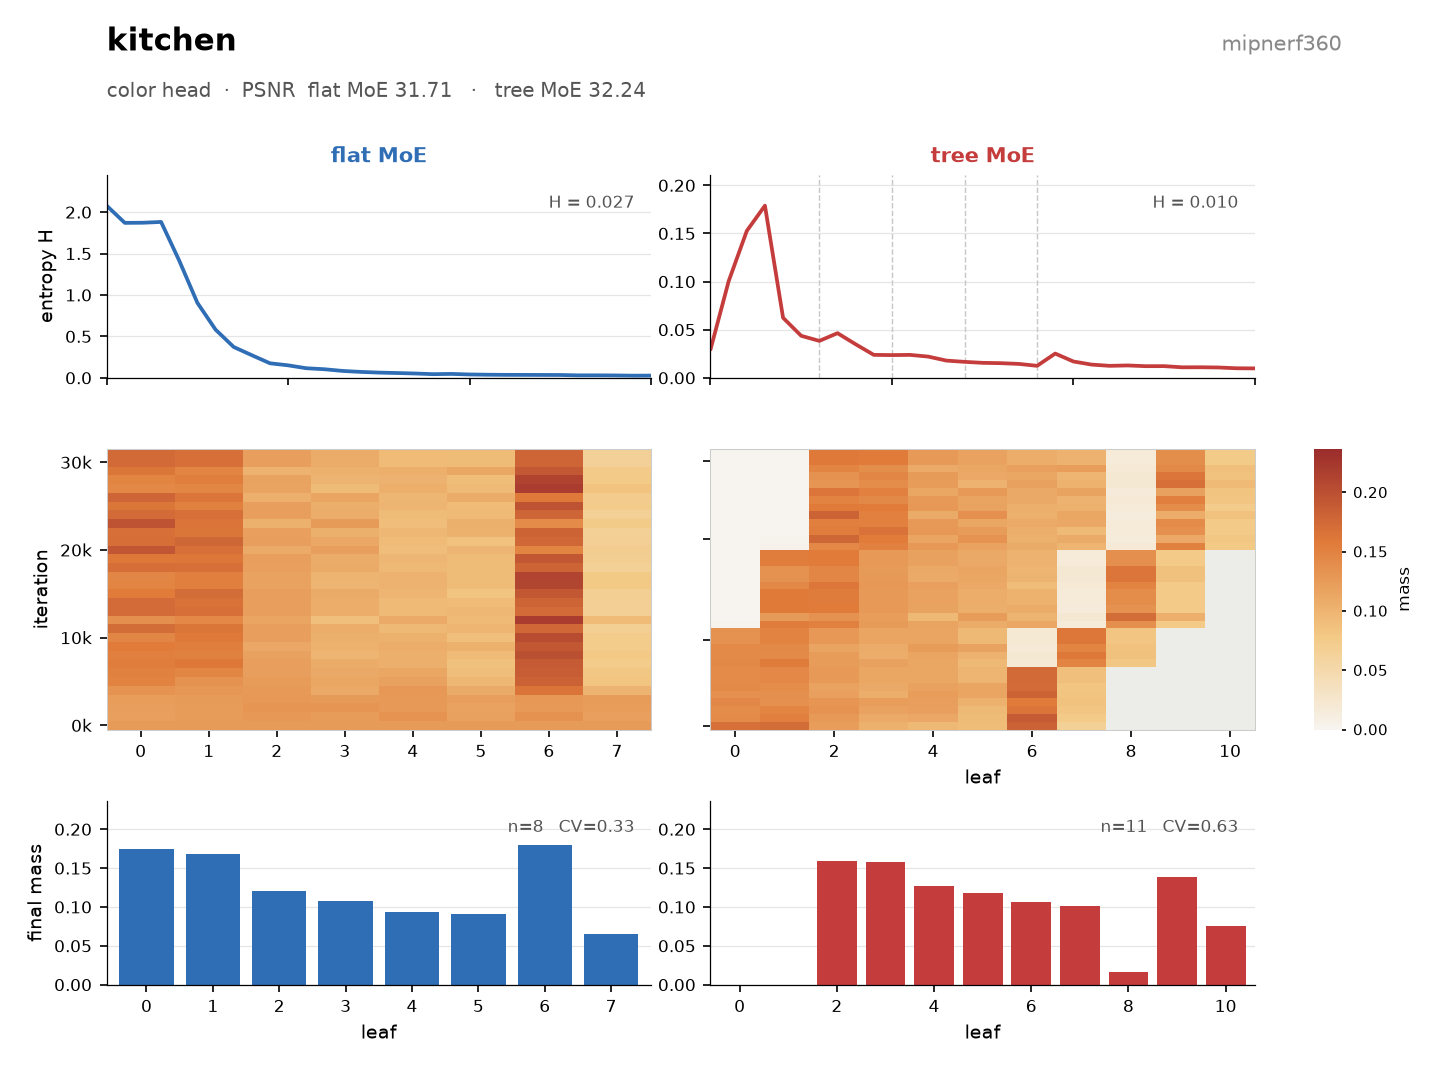
\includegraphics[width=\linewidth]{figures/kitchen.png}
  \caption{\textbf{Per-scene routing dump on \texttt{kitchen}.}
  Columns: flat MoE, tree MoE (color head).
  Top: sample entropy. Middle: leaf mass over training
  (gray \(=\) not yet grown). Bottom: final mass, leaf count \(n\), and
  utilization CV.}
  \label{fig:app-kitchen}
\end{figure}

\subsection{Final entropy and utilization}
\label{app:routing-final}

Figure~\ref{fig:app-hcv} summarizes the 30k color-head statistics on all
19 scenes. Tree MoE has \emph{lower} sample entropy than flat MoE on every
scene, even though it has more leaves (11 vs.\ 8): the extra capacity is
used as specialists, not as a more uniform mixture.
Utilization CV is mixed and should not be read as ``tree is more balanced.''
Flat MoE is sometimes peaked (\texttt{room}, \texttt{bonsai}, CV \(\ge 0.85\))
and sometimes flatter (\texttt{kitchen}, \texttt{garden}).
Tree CV lies in a narrower band, roughly \(0.5\)--\(0.7\), because splits
move mass onto children and leave some parents empty.

Opacity routers stay slightly higher-entropy than color; covariance
collapses first. We therefore report color in the main paper as the head
that actually paints the image.

\begin{figure}[t]
  \centering
  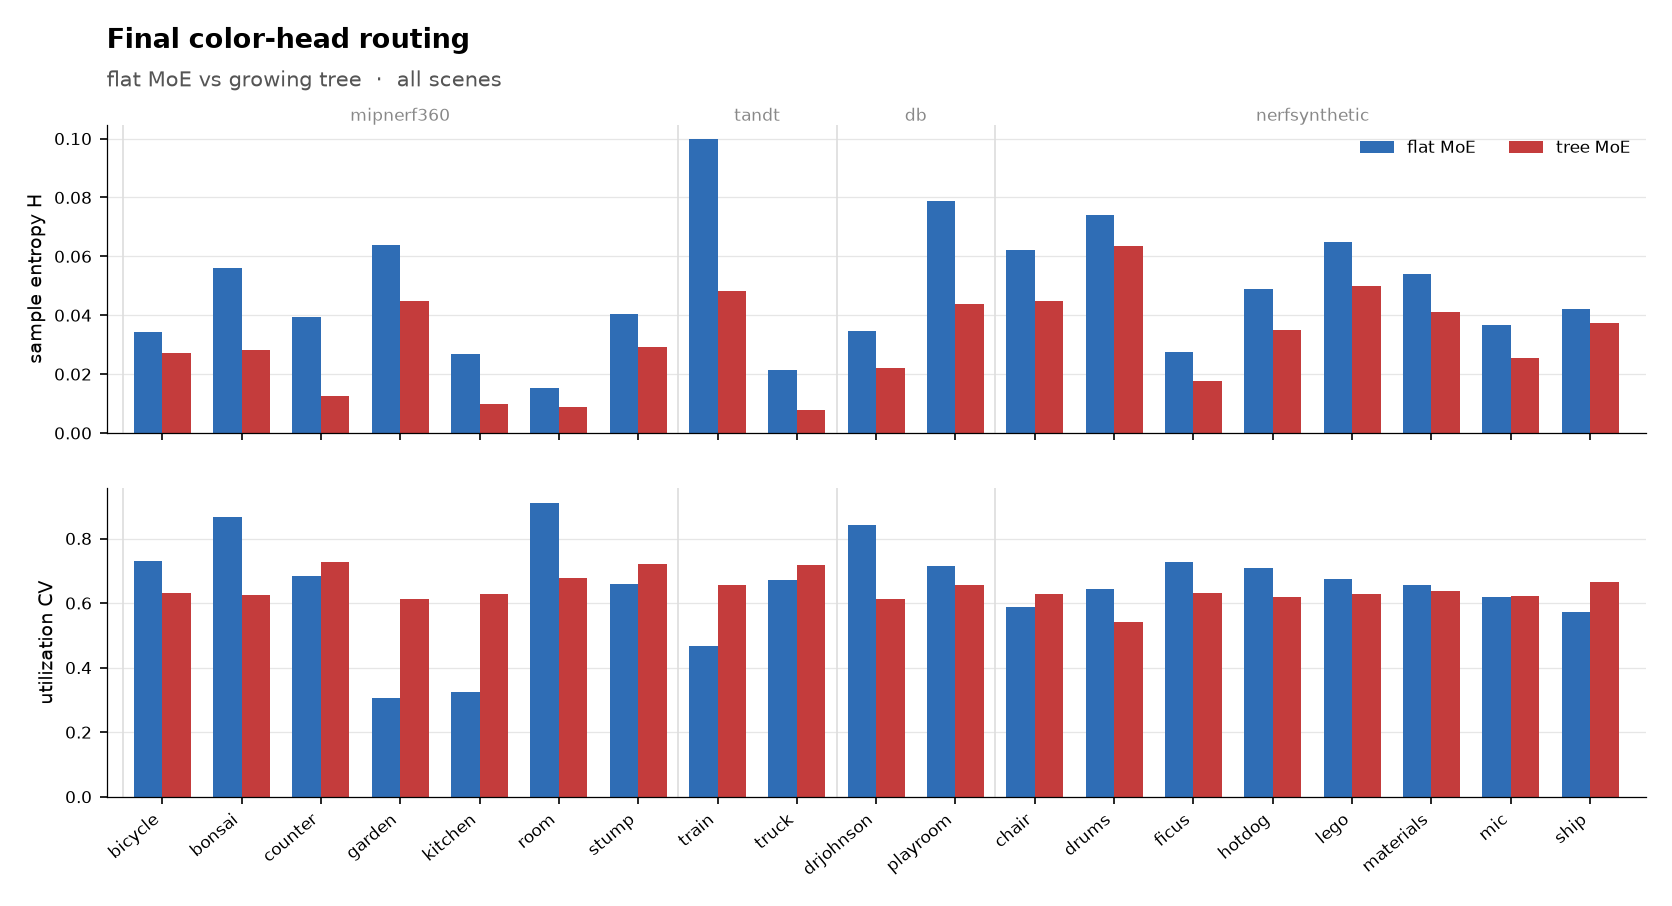
\includegraphics[width=\linewidth]{figures/all_scenes__final_metrics.png}
  \caption{\textbf{Final color-head entropy and utilization CV} (19 scenes).
  Top: sample entropy \(H\); tree \(<\) flat on every scene.
  Bottom: utilization CV (0 \(=\) equal mass). Tree CV is steadier;
  flat MoE oscillates between collapse and near-uniform use of the 8 experts.}
  \label{fig:app-hcv}
\end{figure}

These traces are consistent with Sec.~\ref{sec:grow-ablate}:
\(G_{\max}{=}0\) already captures most of the PSNR gain.
Growth reallocates capacity and makes that specialization readable;
it is not required for the mean \(+0.30\)\,dB over flat MoE.
.

\section{Additional routing analysis}
\label{app:routing}

The main paper reports only the \emph{final} color-leaf mass heatmap.
This appendix records how that assignment is reached: gate entropy over
training, a single-scene growth trace, and final entropy / utilization
statistics. All plots use the color head.
Logs are written every 1k iterations to \texttt{routing\_analysis.json}.
Sample entropy \(H\) is in nats (uniform over 8 experts is \(\ln 8 \approx 2.08\)).

\subsection{Entropy over training}
\label{app:routing-entropy}

Figure~\ref{fig:app-entropy} shows color-head sample entropy versus
iteration on Mip-NeRF~360. Flat MoE uses a dense softmax for the first
\(T_{\mathrm{w}}{=}3000\) iterations, so \(H\) sits near \(2.08\), then
collapses after Top-2 turns on. Tree MoE is warm-started from the Stage~A
checkpoint, so it never revisits that dense plateau: \(H\) stays near zero,
with a small bump at the start of Stage~B and faint rises after grow
checks (dashed, \(t\in\{6\mathrm{k},10\mathrm{k},14\mathrm{k},18\mathrm{k}\}\)).
The same curves on Tanks~\&~Temples, Deep Blending, and NeRF-Synthetic
are Figs.~\ref{fig:entropy-tandt}--\ref{fig:entropy-nerf}.
\texttt{train} keeps the highest residual flat-MoE entropy (\(H{=}0.100\));
the tree still halves it.

\begin{figure}[t]
  \centering
  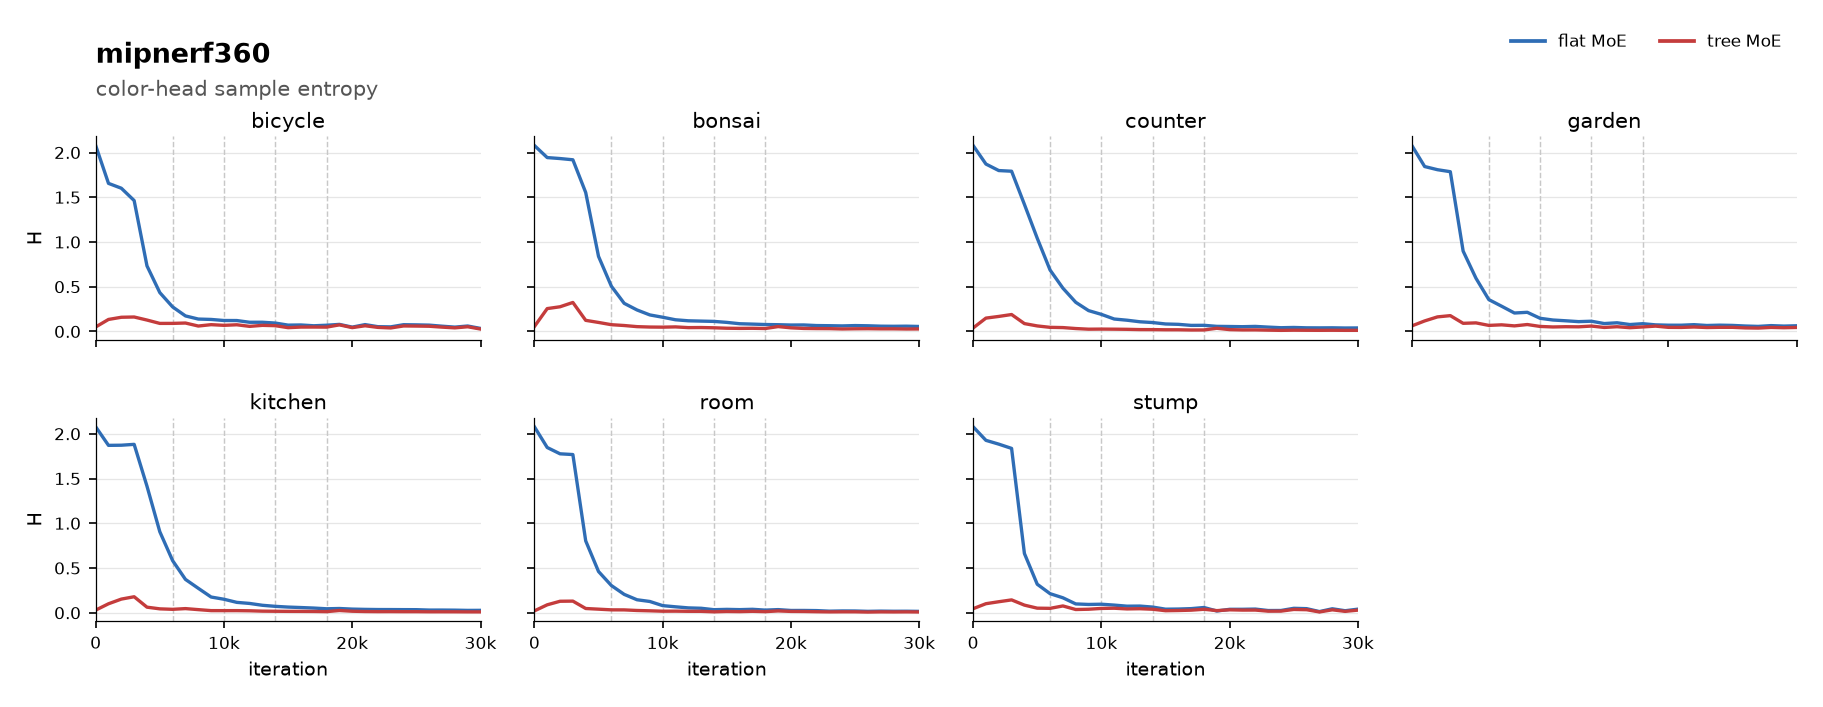
\includegraphics[width=\linewidth]{figures/mipnerf360__entropy_grid.png}
  \caption{\textbf{Color-head sample entropy over training} (Mip-NeRF~360).
  Blue: flat MoE. Red: tree MoE. Shared \(y\)-axis.
  Flat MoE shows the dense-warmup plateau then a Top-2 collapse;
  tree MoE remains specialized throughout Stage~B.}
  \label{fig:app-entropy}
\end{figure}

\begin{figure}[t]
  \centering
  \includegraphics[width=\linewidth]{tandt__entropy_grid.png}
  \caption{Color-head sample entropy \(H\) versus iteration on Tanks~\&~Temples
  (\texttt{train}, \texttt{truck}).
  Blue: flat MoE (dense softmax for \(3\mathrm{k}\) iterations, then Top-2).
  Red: tree MoE warm-started from Stage~A; dashed lines are growth checks.
  Flat MoE collapses after warm-up; tree MoE stays near \(H{\approx}0\).
  \texttt{train} is the slowest collapse and the highest residual entropy.}
  \label{fig:entropy-tandt}
\end{figure}

\begin{figure}[t]
  \centering
  \includegraphics[width=\linewidth]{db__entropy_grid.png}
  \caption{Color-head sample entropy \(H\) versus iteration on Deep Blending
  (\texttt{drjohnson}, \texttt{playroom}).
  Blue: flat MoE. Red: tree MoE. Shared \(y\)-axis in nats
  (uniform over 8 experts is \(\ln 8\approx 2.08\)).
  Both indoor scenes follow the same curriculum: a dense-warmup plateau,
  then a Top-2 collapse.
  Tree MoE never revisits that plateau; \texttt{playroom} keeps a slightly
  higher residual \(H\) than \texttt{drjohnson}.}
  \label{fig:entropy-db}
\end{figure}

\begin{figure}[t]
  \centering
  \includegraphics[width=\linewidth]{nerfsynthetic__entropy_grid.png}
  \caption{Color-head sample entropy \(H\) versus iteration on all eight
  NeRF-Synthetic scenes.
  Blue: flat MoE. Red: tree MoE.
  Every object shows the same pattern as the real scenes: flat MoE sits near
  \(H{\approx}2\) during warm-up and then specializes, while tree MoE remains
  specialized for the whole \(30\mathrm{k}\) Stage~B run.}
  \label{fig:entropy-nerf}
\end{figure}

\subsection{Growth trace on \texttt{kitchen}}
\label{app:routing-kitchen}

Figure~\ref{fig:app-kitchen} is the per-scene dump for \texttt{kitchen}
(\(+1.00\)\,dB vs.\ Scaffold-GS, \(+0.53\)\,dB vs.\ flat MoE).
The middle row is routing mass versus iteration.
Gray cells are leaves that do not exist yet; new columns appear at grow
events. After a split the parent goes dark and the two children inherit
its mass. On \texttt{kitchen} the color head splits \(L_{6,7}\) at 6k and
\(L_{0,1}\) at 10k, ending at 11 leaves, one of which is unused.
The top row is entropy (baseline is the shared MLP, \(H{=}0\));
the bottom row is the 30k mass histogram (same information as one row of
the main heatmap). Bonsai is the other high-gain scene and shows a
stronger flat-MoE collapse (CV \(0.87\), two experts hold most of the mass).

\begin{figure}[t]
  \centering
  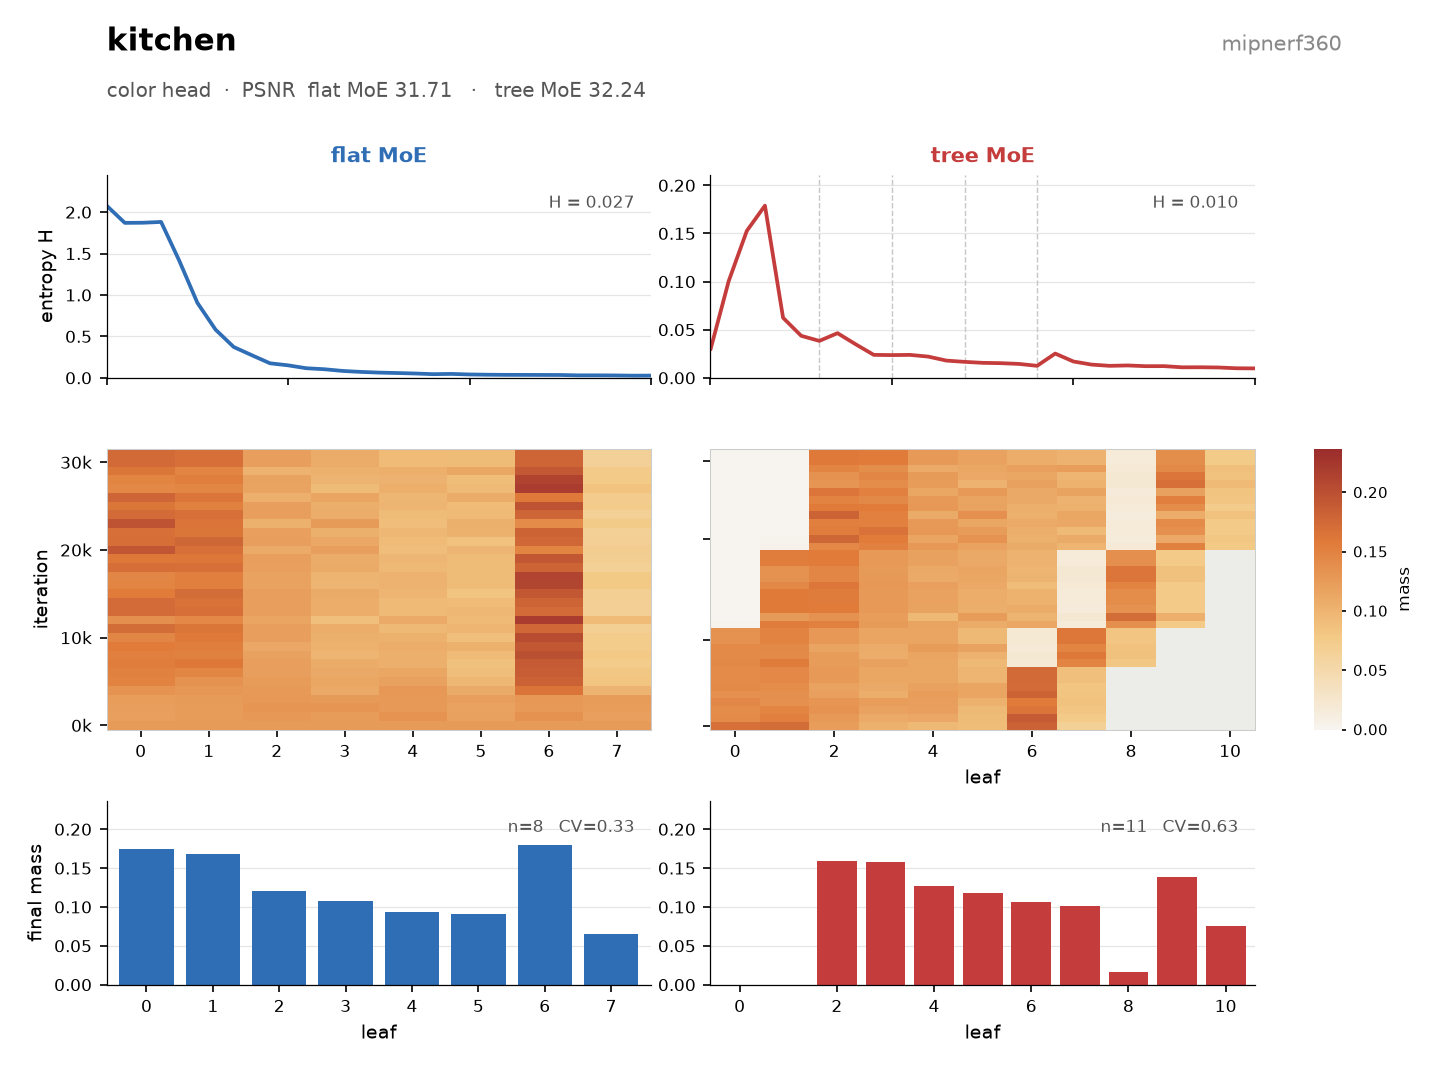
\includegraphics[width=\linewidth]{figures/kitchen.png}
  \caption{\textbf{Per-scene routing dump on \texttt{kitchen}.}
  Columns: flat MoE, tree MoE (color head).
  Top: sample entropy. Middle: leaf mass over training
  (gray \(=\) not yet grown). Bottom: final mass, leaf count \(n\), and
  utilization CV.}
  \label{fig:app-kitchen}
\end{figure}

\subsection{Final entropy and utilization}
\label{app:routing-final}

Figure~\ref{fig:app-hcv} summarizes the 30k color-head statistics on all
19 scenes. Tree MoE has \emph{lower} sample entropy than flat MoE on every
scene, even though it has more leaves (11 vs.\ 8): the extra capacity is
used as specialists, not as a more uniform mixture.
Utilization CV is mixed and should not be read as ``tree is more balanced.''
Flat MoE is sometimes peaked (\texttt{room}, \texttt{bonsai}, CV \(\ge 0.85\))
and sometimes flatter (\texttt{kitchen}, \texttt{garden}).
Tree CV lies in a narrower band, roughly \(0.5\)--\(0.7\), because splits
move mass onto children and leave some parents empty.

Opacity routers stay slightly higher-entropy than color; covariance
collapses first. We therefore report color in the main paper as the head
that actually paints the image.

\begin{figure}[t]
  \centering
  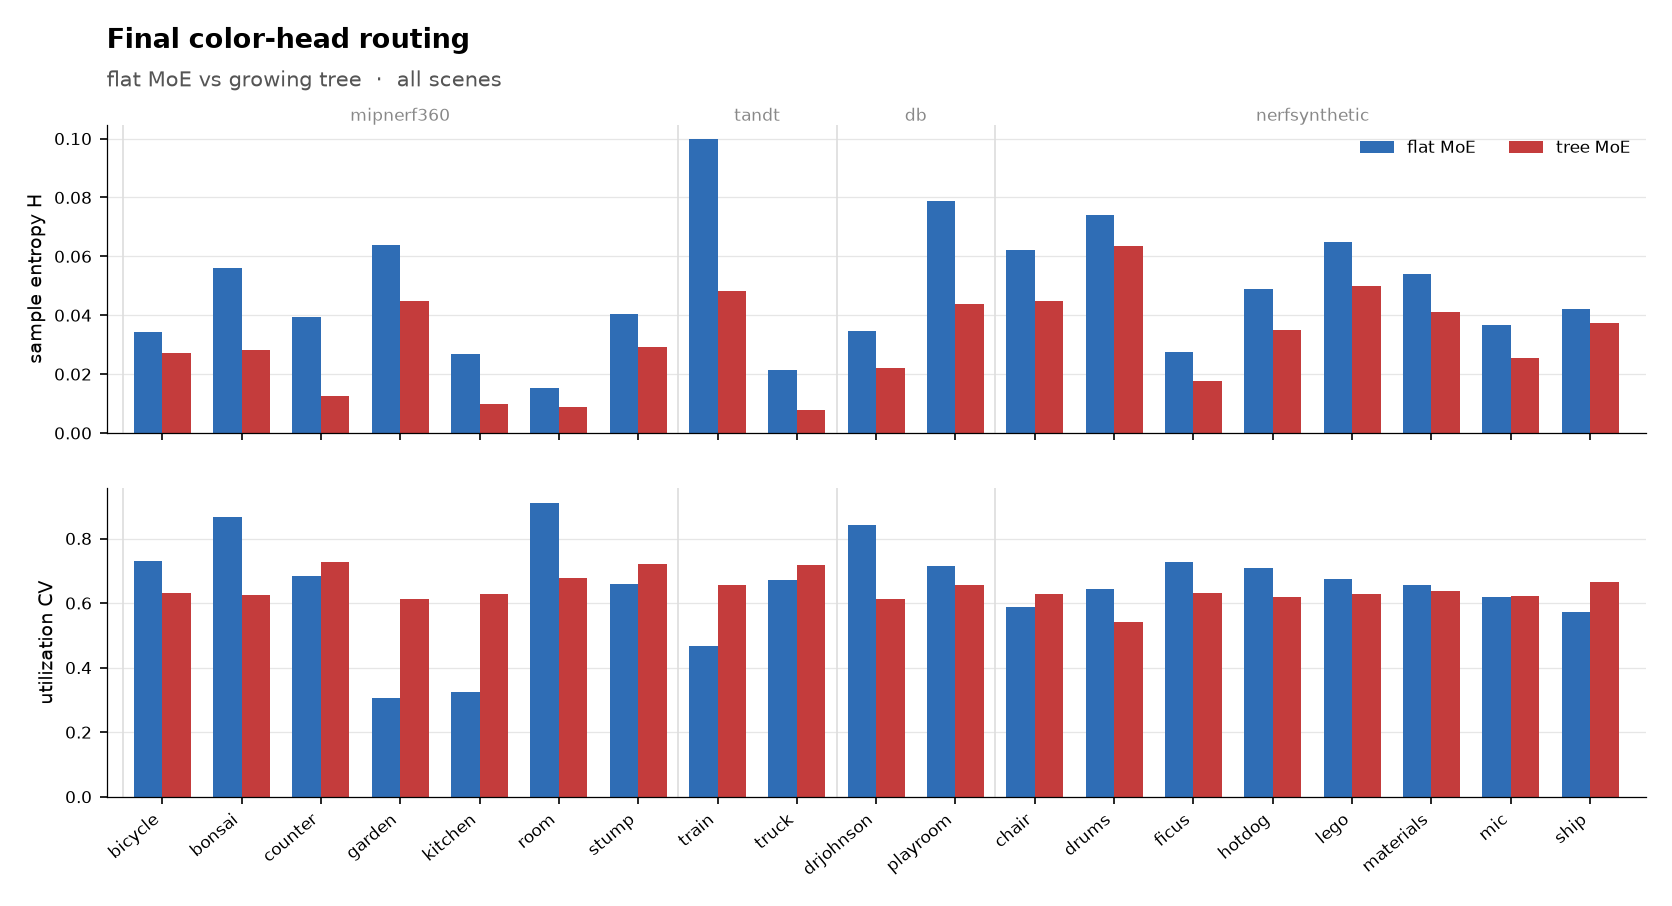
\includegraphics[width=\linewidth]{figures/all_scenes__final_metrics.png}
  \caption{\textbf{Final color-head entropy and utilization CV} (19 scenes).
  Top: sample entropy \(H\); tree \(<\) flat on every scene.
  Bottom: utilization CV (0 \(=\) equal mass). Tree CV is steadier;
  flat MoE oscillates between collapse and near-uniform use of the 8 experts.}
  \label{fig:app-hcv}
\end{figure}

These traces are consistent with Sec.~\ref{sec:grow-ablate}:
\(G_{\max}{=}0\) already captures most of the PSNR gain.
Growth reallocates capacity and makes that specialization readable;
it is not required for the mean \(+0.30\)\,dB over flat MoE.
